\section{Potentiale}\label{sec:Potentiale}

Eine Schwierigkeit bei der Analyse von Spielen bildet der Umstand, dass jeder Spieler eine eigene Kostenfunktion und damit ein eigenes Optimierungsziel hat. Möchte man also beispielsweise Gleichgewichtspunkte finden, so muss man alle diese Funktionen gleichzeitig (lokal) optimieren. Diese Aufgabe wird wesentlich einfacher, wenn das Spiel eine sogenannte Potentialfunktion besitzt. Eine solche ist eine Funktion auf dem Strategieraum des Spieles, die ein alternatives Koordinationsspiel darauf definiert, welches gewisse Eigenschaften mit dem ursprünglichen Spiel teilt (etwa die Lage der Gleichgewichtspunkte).

In diesem Kapitel werden wir einige Varianten von Potentialfunktionen kennenlernen und feststellen, welche Spiele diese jeweils besitzen. In \Cref{sec:Morphismen} werden wir dann die Beziehung zwischen Ausgangsspiel und dem von einer Potentialfunktion beschriebenen Koordinationsspiel durch Morphismen beschreiben und dadurch zeigen, welche Eigenschaften beim Wechsel zwischen den beiden Spielen erhalten bleiben.

\subsection{Definitionen}

Zunächst definieren wir eine Auswahl verschiedener Typen von Potentialfunktionen:

\begin{defn}
	Zu einem Spiel $\Gamma = (I, X, (c_i)_{i\in I})$ heißt eine Funktion $P: X \to \IR$
	\begin{itemize}
		\item \emph{verallgemeinertes Nash-Potential}, wenn jedes Minimum von $P$ ein Nash-Gleichgewicht in $\Gamma$ ist, d.h. für alle $x \in X$ gilt:
			\[P(x) = \min_{\hat{x} \in X}P(\hat{x}) \implies \forall i \in I, \hat{x}_i \in X_i: c_i(x) \leq c_i(x \mid \hat{x}_i) \]
		\item \emph{Nash-Potential}, wenn jedes Minimum von $P$ ein Nash-Gleichgewicht in $\Gamma$ ist und umgekehrt, d.h. für alle $x \in X$ gilt:
			\[P(x) = \min_{\hat{x} \in X}P(\hat{x}) \iff \forall i \in I, \hat{x}_i \in X_i: c_i(x) \leq c_i(x \mid \hat{x}_i) \]
		\item \emph{lokales Nash-Potential}, wenn jedes lokale Minimum von $P$ ein Nash-Gleichgewicht in $\Gamma$ ist und umgekehrt, d.h. für alle $x \in X$ gilt:
			\[\forall i \in I, \hat{x}_i \in X_i: P(x) \leq P(x \mid \hat{x}_i) \iff \forall i \in I, \hat{x}_i \in X_i: c_i(x) \leq c_i(x \mid \hat{x}_i) \]
		\item \emph{Beste-Antwort-Potential}, wenn für jeden Spieler $i$ und alle Strategieprofile $x \in X$ gilt:
			\[\arg\min_{\hat{x}_i \in X_i}c_i(x \mid \hat{x}_i) = \arg \min_{\hat{x}_i \in X_i} P(x \mid \hat{x}_i)\]
		\item \emph{verallgemeinertes ordinales Potential}, wenn für jeden Spieler $i$ und alle Strategieprofile $x \in X$ sowie $\hat{x}_i \in X_i$ gilt:
			\[c_i(x) > c_i(x \mid \hat{x}_i) \implies P(x) > P(x \mid \hat{x}_i)\]
		\item \emph{ordinales Potential}, wenn für jeden Spieler $i$ und alle Strategieprofile $x \in X$ sowie $\hat{x}_i \in X_i$ gilt:
			\[c_i(x) > c_i(x \mid \hat{x}_i) \iff P(x) > P(x \mid \hat{x}_i)\]
		\item \emph{skaliertes Potential}, wenn es streng monotone Funktionen $f_i: \IR \to \IR$ gibt, sodass für jeden Spieler $i$ und alle Strategieprofile $x \in X$ sowie $\hat{x}_i \in X_i$ gilt:
			\[c_i(x) - c_i(x \mid \hat{x}_i) = f_i(P(x)) - f_i(P(x \mid \hat{x}_i))\]
		\item \emph{gewichtetes Potential}, wenn es einen Gewichtsvektor $(w_i)_{i\in I} \in \IR_{>0}^I$ gibt, sodass für jeden Spieler $i$ und alle Strategieprofile $x \in X$ sowie $\hat{x}_i \in X_i$ gilt:
			\[c_i(x) - c_i(x \mid \hat{x}_i) = w_i\cdot(P(x) - P(x \mid \hat{x}_i))\]
		\item \emph{exaktes Potential}, wenn für jeden Spieler $i$ und alle Strategieprofile $x \in X$ sowie $\hat{x}_i \in X_i$ gilt:
			\[c_i(x) - c_i(x \mid \hat{x}_i) = P(x) - P(x \mid \hat{x}_i)\]
		\item \todo[inline]{Potentiale aus \cite{BestRespEq}?}
	\end{itemize}
\end{defn}

Exakte, gewichtete, ordinale und verallgemeinerte ordinale Potentiale wurden erstmals in \cite{MonShap} definiert, beste Antwort-Potentiale erstmals in \cite{BestRespPot}. Die Beziehungen zwischen den verschiedenen Potentialbegriffen werden in folgendem an \cite{BestRespPot} angelehnten Euler-Diagramm (\Cref{diag:Potentiale}) dargestellt:

\begin{figure}[h]\centering
	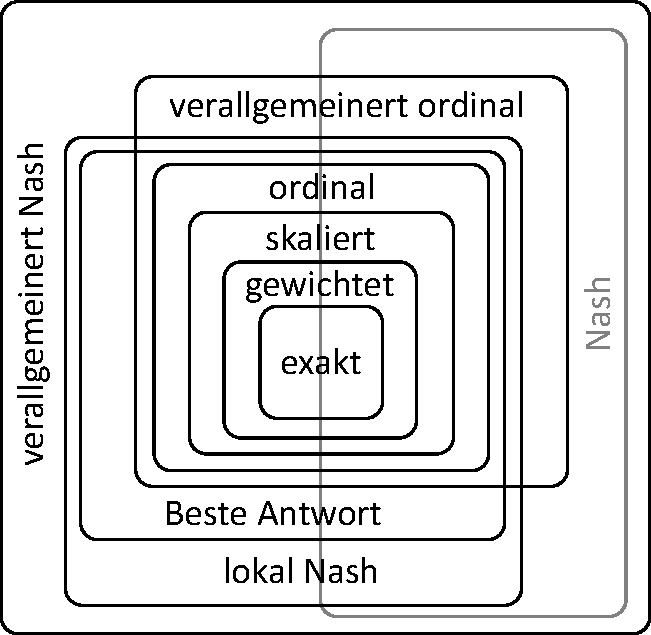
\includegraphics[width=.4\textwidth]{../Bilder/EulerDiagPotentiale.pdf}
	\caption{Beziehungen zwischen den einzelnen Potentialbegriffen}\label{diag:Potentiale}
\end{figure}

\todo[inline]{Beziehungen beweisen? $\rightarrow$ Kapitel 3}

\todo[inline]{Wann ist ein ordinales Potentialspiel bereits ein skaliertes? Zumindest für endliche Spiele sollte das stimmen?}

\begin{bsp}
	Jedes Koordinationsspiel besitzt ein exaktes Potential (nämlich die gemeinsame Kostenfunktion). Ebenso besitzt jedes Dummyspiel ein exaktes Potential (nämlich die konstante $0$-Funktion).
	
	Entsprechend besitzt jedes skalierte Koordinationsspiel ein skaliertes Potential.
\end{bsp}

\subsection{Anschauung}

Verallgemeinerte Nash-Potentiale (und damit alle oben beschriebenen Potentiale) formalisieren die Idee ein Spiel durch irgendein anderes durch eine einzige Funktion beschriebenes Optimierungsproblem zu ersetzen, dessen Optima Nash-Gleichgewichte im ursprünglichen Spiel sind. Im Falle eines Nash-Potentials entsprechen diese Optima sogar allen Nash-Gleichgewichten. Findet man nun ein solches Optimierungsproblem, von dem man zeigen kann, dass es immer ein Optimum besitzt (etwa weil es durch eine stetige Funktion beschrieben wird und der Strategieraum kompakt ist), so zeigt dies, dass das ursprüngliche Spiel mindestens ein Nash-Gleichgewicht besitzt. Außerdem kann man dieses durch Lösen des Optimierungsproblems bestimmen.

Versteht man zu einem gegebenen Strategieprofil $x \in X$ dessen \emph{Nachbarschaft} als die Menge aller durch höchstens eine Abweichung erreichbarer Strategieprofile, d.h. die Menge $\{(x \mid \hat{x}_i) | i \in I, \hat{x}_i \in X_i\}$, so nennen wir $x$ ein \emph{lokales Minimum} einer Funktion $P: X \to \IR$, wenn es ein Minimum innerhalb seiner Nachbarschaft ist.\todo{Evtl. diese Definition zusammen mit einer Erwähnung zum Zusammenhang mit lokaler Suche bereits in das Grundlagenkapitel verschieben?}{} Ein lokales Nash-Potential beschreibt damit ein Optimierungsproblem, dessen \emph{lokale} Minima den Nash-Gleichgewichten des Ausgangsspiels entsprechen.

Die Nachbarschaft eines Strategieprofils $x$ besteht nun gerade aus den Profilen, die man mit $x$ vergleichen muss, um festzustellen, ob es sich bei $x$ um ein Nash-Gleichgewicht handelt. Hat man also ein Spiel $\Gamma = (I, X, (c_i))$ mit einem lokalen Nash-Potential $P$, so induziert dieses ein Koordinationsspiel $K \coloneqq (I, X, (P))$ auf dem selben Strategieraum, dessen Nash-Gleichgewichte gerade mit denen des Spiels $\Gamma$ übereinstimmen.

Weitere Spezialisierungen dieses Potentialbegriffs führen dann zu induzierten \todo{Silbentrennung?} Koordinationsspielen, welche noch weitere Eigenschaften des Ausgansspiels übernehmen: So hat das durch ein Beste-Antwort-Potential beschriebene Spiel etwa die gleichen Beste-Antwort-Pfade und eignet sich daher beispielsweise zur Analyse von Beste-Antwort-Dynamiken. Durch ein ordinales Potential erhält man ein Spiel, welches auch die gleichen Verbesserungs- und Nichtverschlechterungspfade enthält. Bei einem verallgemeinerten ordinalen Potential bleiben diese hingegen jeweils nur in eine Richtung erhalten: Ein Verbesserungspfad im Ausgangsspiel ist auch einer im Koordinationsspiel und ein Nichtverschlechterungspfad im Koordinationsspiel entspricht einem solchen im ursprünglichen Spiel.\todo{Stimmt das?}

Für skalierte, gewichtete und exakte Potentiale gibt es eine noch anschaulichere Betrachtungsweise für den Fall (endlicher) 2-Personenspiele. Deren Strategieraum kann man als Gitternetz in der Ebene auffassen, wobei jede Strategie von Spieler 1 einer senkrechten und jede Strategie von Spieler 2 einer waagerechten Gitterlinie entspricht. Kreuzungspunkte von zwei Gerade entsprechen dann gerade vollständige Strategieprofilen. Kostenfunktionen (ebenso wie Potentiale) sind dann \glqq Reliefkarten\grqq{}, deren Höhe den jeweiligen Kosten entspricht. 

\begin{figure}[h]\centering
	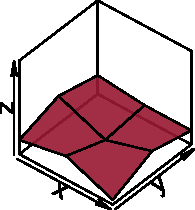
\includegraphics[width=.3\textwidth]{../Bilder/exaktesPotentialSp1.pdf}
	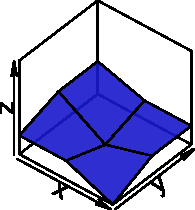
\includegraphics[width=.3\textwidth]{../Bilder/exaktesPotentialSp2.pdf}
	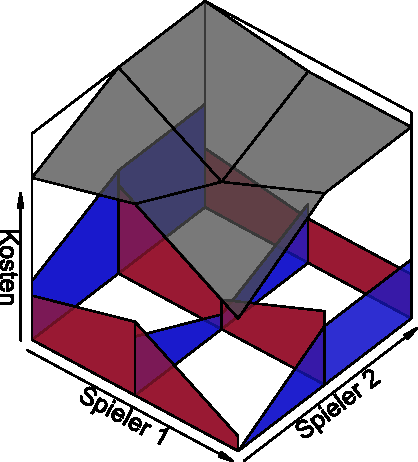
\includegraphics[width=.3\textwidth]{../Bilder/exaktesPotential.pdf}
	\caption{Ein 2-Personenspiel mit exaktem Potential (grau): Spieler 1: rot, Spieler 2: blau}
\end{figure}

Ein exaktes Potential entspricht in diesem Bild einer gemeinsamen Reliefkarte für beide Spieler, die - im Falle eines exakten Potentials - \glqq scheibenweise\grqq{} bis auf eine additive Konstante mit der eigentlichen Kostenfunktion übereinstimmt. Anders formuliert: Wird die Strategie eines Spieler festgehalten, so kann der andere Spieler seine Kostenveränderungen bei der Wahl der verschiedenen ihm zur Verfügung stehenden Strategien auch anhand der Potentialfunktion ablesen. 

Geht man nun über zu einem skalierten Potential, so lesen die beiden Spieler das Potential sozusagen in verschiedenen Einheiten. Sind die Skalierungsfunktionen linear (das Potential also sogar ein gewichtetes), dann sind die verschiedenen Einheiten proportional zueinander.\todo{Alternativ direkt sagen, dass das Potentialrelief verschieden stark gestreckt/gestaucht wird.} 


\subsection{Eigenschaften der Potentiale}

Wir wollen hier noch einige Eigenschaften der verschiedenen Potentiale zusammenfassen - beweisen werden wir sie dann aber erst in \Cref{sec:Morphismen}.

\begin{beob}\label{beob:lokMinNG}
	Ist $\Gamma$ ein Spiel mit einem lokalen Nash-Potential $P$. Dann ist jedes lokale Minimum von $P$ ein Nash-Gleichgewicht von $\Gamma$ und umgekehrt.\todo{Eigentlich ist das für dieses Potential gar kein Satz, sondern einfach die Definition}
\end{beob}

Diese Beobachtung zeigt also, dass man Nash-Gleichgewichte allein durch Betrachten einer Potentialfunktion finden kann. Daraus folgt direkt die Existenz von Nash-Gleichgewichten in einer Vielzahl von Potentialspielen, nämlich all diejenigen deren Potentialfunktion mindestens ein globales (und damit erst recht lokales) Minimum haben. Also beispielsweise:

\begin{kor}
	Sei $\Gamma$ ein Spiel mit einem kompakten Strategieraum und einer stetigen lokalen Nash-Potentialfunktion. Dann hat $\Gamma$ wenigstens ein Nash-Gleichgewicht.
\end{kor}

Insbesondere also haben endliche Potentialspiele immer ein Nashgleichgewicht. 

\begin{satz}\label{prop:ordPotVerbpfad}
	Sei $\Gamma$ ein Spiel mit einem verallgemeinerten ordinalen Potential $P$. Dann ist jeder Verbesserungspfad in $\Gamma$ auch ein Verbesserungspfad bezüglich $P$. Ist $P$ sogar ein ordinales Potential, so gilt auch die umgekehrte Richtung.
\end{satz}

Zusammen mit \Cref{kor:ExVerbPfadExNG} werden wir hieraus später folgern, dass ordinale Potentiale lokale Nash-Potentiale sind. Ferner ergibt sich daraus, dass ein lokales Minimum eines verallgemeinerten ordinalen Potentials ein Nash-Gleichgewicht des eigentlichen Spiels ist. Die Umkehrung gilt in diesem Fall aber nicht mehr notwendigerweise.\todo{Beispiel?}

Analog zu diesem Satz gilt für Beste-Antwort-Pfade und Beste-Antwort-Potentiale:

\begin{satz}\label{prop:BAPotBAPad}
	Sei $\Gamma$ ein Spiel mit einem Beste-Antwort-Potential $P$. Dann ist jeder Beste-Antwort-(Verbesserungs-)Pfad in $\Gamma$ auch ein Beste-Antwort-(Verbesserungs-)Pfad bezüglich $P$ und umgekehrt.
\end{satz}

Und auch hieraus erhalten wir mit \Cref{kor:ExVerbPfadExNG}, dass Beste-Antwort-Potentiale lokale Nash-Potentiale sind. \Cref{tab:PotErhalten} fasst einige der von Potentialen erhaltenen Eigenschaften zusammen.

\begin{table}[h]\centering
	\begin{tabular}{l|ccccc}
						& Nash-Gl. 			& FIP 					& Nichtverschl.pfad 			& Verb.pfad 		& Beste-Antwort-Pfad \\\hline
		exakt			& $\Leftrightarrow$	& $\Leftrightarrow$ 	& $\Leftrightarrow$				& $\Leftrightarrow$	& $\Leftrightarrow$ \\
		gewichtet		& $\Leftrightarrow$	& $\Leftrightarrow$ 	& $\Leftrightarrow$				& $\Leftrightarrow$	& $\Leftrightarrow$ \\		
		skaliert		& $\Leftrightarrow$ & $\Leftrightarrow$ 	& $\Leftrightarrow$				& $\Leftrightarrow$	& $\Leftrightarrow$ \\
		ordinal			& $\Leftrightarrow$	& $\Leftrightarrow$ 	& $\Leftrightarrow$				& $\Leftrightarrow$	& $\Leftrightarrow$ \\
		verallg. ordinal& $\Leftarrow$		& $\Rightarrow$		 	& $\Leftarrow$					& $\Rightarrow$		& $\Rightarrow$ 	\\
		Beste Antwort	& $\Leftrightarrow$	& 					 	& 								& 					& $\Leftrightarrow$ \\
		lokal Nash		& $\Leftrightarrow$	& 					 	& 								& 					& 					
	\end{tabular}	
	\caption{Welche Eigenschaft bleibt beim Übergang von einem Spiel auf das von einem entsprechenden Potential induzierte Koordinationsspiel erhalten ($\Rightarrow$) und welche bei der umgekehrten Richtung ($\Leftarrow$)?\\\todo[inline]{Tabelle korrigieren, erweitern, erklären...}}\label{tab:PotErhalten}
\end{table}

Für Spiele mit unendlicher Spielermenge wird sich im folgenden Abschnitt die Beobachtung als hilfreich erweisen, dass wir die meisten Potentiale pfadzusammenhangskomponentenweise definieren können:

\begin{beob}\label{beob:KompWeisePotentiale}
	Sei $\Gamma$ ein beliebiges Spiel und $P: X \to \IR$ eine Funktion. Erfüllt $P$ dann die Bedingung eines exakten/gewichteten/skalierten/ordinalen/verallgemeinerten ordinalen/Beste Antwort/lokalen Nash-Potentials für jede (maximale) Pfadzusammenhangskomponente, so ist $P$ ein entsprechendes Potential für ganz $\Gamma$.
\end{beob}

\begin{proof}
	Dies folgt direkt aus dem Umstand, dass die definierende Eigenschaft für alle aufgezählten Potentiale immer nur entlang eines Pfades (der Länge $1$) und damit innerhalb einer Zusammenhangskomponente geprüft werden muss.
\end{proof}


\subsection{Charakterisierungen der Potentiale}

In diesem Abschnitt wollen wir für einige der zuvor beschriebenen Potentiale notwendige und hinreichende Anforderungen an ein Spiel beschreiben, damit dieses ein entsprechendes Potential besitzt.

\subsubsection{Exakte Potentiale}

\begin{satz}\label{satz:CharExPot}
	Ein Spiel besitzt genau dann ein exaktes Potential, wenn alle 4-Zykel im Strategieraum eine Gesamtänderung von $0$ haben.
\end{satz}

\begin{proof}
	Wir folgen dem Beweis aus \cite[Anhang A]{MonShap}. Dort wird der Satz zwar nur für $N$-Personenspiele gezeigt, mit \Cref{beob:KompWeisePotentiale} überträgt sich dieser Beweis aber direkt auch auf allgemeine Spiele.
	
	Sei zunächst $\gamma \coloneqq (x^0, x^1, x^2, x^3, x^4)$ ein beliebiger 4-Zykel in einem Spiel mit Potential $P$. Dann gilt für die Gesamtänderung:
		\[\PfadAend(\gamma) = \sum_{i=1}^4 \left(c_{i(k)}(x^k) - c_{i(k)}(x^{k-1})\right) = \sum_{k=1}^{4} \left(P(x^k) - P(x^{k-1})\right) = P(x^4) - P(x^0) = 0^{}\]
		
	Ist umgekehrt $\Gamma$ ein Spiel, in dem für alle 4-Zykel $\gamma$ gilt $\PfadAend(\gamma) = 0$, $x$ ein beliebiges, aber festes Strategieprofil in $\Gamma$ und $Y_x$ dessen Pfadzusammenhangskomponente, dann definiere wie folgt eine Funktion $P_x$ auf $Y_x$:
		\[P: Y_x \to \IR: y \mapsto \PfadAend(\gamma), \,\gamma \text{ beliebiger Pfad von } x \text{ nach } y \]
	Damit diese Funktion tatsächlich wohldefiniert ist, muss für je zwei Pfade $\gamma$ und $\gamma'$ von $\hat{x}$ nach $x$ gelten, dass die jeweiligen Gesamtänderungen gleich sind, d.h. $\PfadAend(\gamma) = \PfadAend(\gamma')$. Dies ist äquivalent dazu, dass der Zykel, den man durch Verknüpfen der beiden Pfade $\gamma$ und $\overset{\leftarrow}{\gamma'}$ erhält eine Gesamtänderung von $0$ hat. Dazu zeigen wir nun mittels Induktion über deren Länge, dass für alle Zykel $\mu$ gilt $\PfadAend(\mu) = 0$:
	\begin{description}
		\item[IA ($\bm{\abs{\mu}=4}$)\footnote{Zykel der Längen $0$, $2$ und $3$ haben automatisch immer Gesamtänderung $0$, da in ihnen alle Abweichungen vom gleichen Spieler vorgenommen werden müssen.}] D.h. $\mu$ ist ein 4-Zykel und damit $\PfadAend(\mu) = 0$ nach Voraussetzung.
		\item[IS ($\bm{\abs{\mu}\eqqcolon n}$)] Vorausgesetzt es gibt einen Pfad $\mu' = (x'^0, \dots, x'^n)$ gleicher Länge und Gesamtänderung wie $\mu$, sodass in den ersten beiden Schritten der gleiche Spieler seine Strategie wechselt, d.h. $i(1)=i(2)$. Dann erhält man durch Weglassen des ersten Schrittes einen \emph{kürzeren} Pfad $\mu'' \coloneqq (x'^0, x'^2, \dots, x'^n)$ mit gleicher Gesamtänderung, welche dann nach Induktion bereits $0$ ist. In diesem Fall haben wir dann wie gewünscht $\PfadAend(\mu) = \PfadAend(\mu') = \PfadAend(\mu'') = 0$.
		
		Die Existenz eines solchen Pfades $\mu'$ zeigen wir nun mittels Induktion über $k \coloneqq \min\left\{1 < l \leq n \setMid i(l) = i(1)\right\}$. Ein solches $k$ existiert immer, da Spieler $i(1)$ bereits im ersten Schritt seine Strategie wechselt und dies daher im Verlauf des Zykels noch mindestens ein weiteres Mal tun muss, damit der Zykel geschlossen werden kann.
		\begin{description}
			\item[IA ($\bm{k=2}$)] Dann gilt bereits $i(1)=i(2)$ und wir sind fertig mit $\mu' \coloneqq \mu$.
			\item[IS ($\bm{k-1\to k}$)] Wir ändern $\mu$ so ab, dass Spieler $i(1)$ bereits im $(k-1)$-ten Schritt der abweichende Spieler ist. Dann sind wir fertig nach Induktionsvoraussetzung. Dazu ersetzen wir in $\mu$ das Strategieprofil $x^k$ durch $(x^{k-1} \mid x^{k+1}_{i(1)})$, sodass also Spieler $i(1)$ bereits einen Schritt früher (im $(k-1)$-ten) seine Strategie wechselt und der Spieler, der dies zuvor in diesem Schritt getan hat, einen Schritt später.
			
			Bei dieser Anpassung bleibt die Gesamtänderung des Pfades $\mu$ gleich, denn wir ersetzen lediglich ein Pfadstück der Länge $2$ durch ein anderes Pfadstück der Länge $2$. Und da sich diese beiden Pfade zu einem 4-Zykel zusammensetzen lassen, haben diese nach Voraussetzung die gleiche Gesamtänderung.
			
			Auf dieses abgeänderte $\mu$ können wir nun die Induktionsvoraussetzung anwenden und erhalten dadurch einen neuen Pfad $\mu'$ mit den gewünschten Eigenschaften.
		\end{description}
		Hiermit können wir auch den Induktionsschritt der äußeren Induktion und damit den Nachweis der Wohldefiniertheit von $P$ abschließen. 
	\end{description}	
	Wählen wir nun für jede maximale Pfadzusammenhangskomponente ein einziges $x$ in dieser und definieren wie oben eine Funktion $P_x$, so lassen sich alle diese Funktionen zu einer Funktion $P$ auf ganz $X$ zusammensetzen. Nach Definition erfüllt diese auf jeder Pfadzusammenhangskomponente die Bedingung eines exakten Potentials. Also ist nach \Cref{beob:KompWeisePotentiale} $P$ ein exaktes Potential auf $X$.
\end{proof}

Eine alternative Charakterisierung für die Existenz eines exakten Potentials zeigt \citeauthor{KoordDummy} in \cite[Theorem 2.1]{KoordDummy}:

\begin{satz}\label{satz:CharExPotAlt}
	Ein Spiel $\Gamma = (I, X, (c_i))$ besitzt genau dann ein exaktes Potential, wenn es ein Koordinationsspiel $K = (I, X, (p))$ und ein Dummy-Spiel $D = (I, X, (d_i))$ auf dem selben Strategieraum gibt, sodass die Kostenfunktionen in $\Gamma$ die Summe der Kostenfunktionen aus $K$ und $D$ sind, d.h. $c_i = p + d_i$.
\end{satz}

\begin{proof}
	Ist $\Gamma$ ein Spiel mit einem exakten Potential $P$, so definiert dieses ein Koordinationsspiel $K \coloneqq (I, X, (P))$. Ferner ist $D \coloneqq (I, X, (P-c_i))$ ein dazu passendes Dummy-Spiel, denn es gilt für jeden Spieler $i \in I$ und alle Strategien/Strategieprofile $x \in X, \hat{x}_i \in X_i$:
		\[(P-c_i)(x) - (P-c_i)(x \mid \hat{x}_i) = \left(P(x) - P(x \mid \hat{x}_i)\right) - \left(c_i(x) - c_i(x \mid \hat{x}_i)\right) = 0 \]
	Also $(P-c_i)(x) = (P-c_i)(x \mid \hat{x}_i)$.
	
	Umgekehrt haben sowohl ein Koordinations- als auch ein Dummy-Spiel ein exaktes Potential. Die Summe der beiden Potentialfunktionen ist dann ein exaktes Potential für die Summe der beiden Spiele.
\end{proof}


\subsubsection{Gewichtete und skalierte Potentiale}

\begin{satz}\label{satz:CharGewPot}
	Ein Spiel besitzt genau dann ein gewichtetes Potential mit Gewichtsvektor $w = (w_i)_{i \in I}$, wenn die $w$-gewichtete Gesamtänderung entlang jedes 4-Zykels $0$ ist, d.h. für jeden 4-Zykel $\gamma \coloneqq (x^0, x^1, x^2, x^3, x^4)$ gilt:\todo{Gibt es eine bessere Charakterisierung von gew. Potentialen? Insb. ohne dass man schon den richtigen Gewichtsvektor angeben muss?}
	\[\PfadAend_w(\gamma) = \sum_{i=1}^4 w_{i(k)}\cdot\left(c_{i(k)}(x^k) - c_{i(k)}(x^{k-1})\right) = 0\]
\end{satz}

Diese Charakterisierung folgt direkt aus der folgenden Beobachtung aus \cite[Kapitel 3.2]{CharExGewPotinWCG}

\begin{beob}\label{beob:ZshExGewPot}
	Zu einem Spiel $\Gamma = (I, X, (c_i))$ ist eine Funktion $P: X \to \IR$ genau dann ein gewichtetes Potential mit Gewichtsvektor $w = (w_i)$, wenn $P$ ein exaktes Potential zum Spiel $\Gamma_w \coloneqq (I, X, (c_i/w_i))$ ist.
\end{beob}

\begin{proof}
	Für jedes Strategieprofil $x \in X$, jeden Spieler $i \in I$ und jede Strategie $\hat{x}_i$ gilt:
		\[c_i(x) - c_i(x \mid \hat{x}_i) = w_i\cdot(P(x) - P(x \mid \hat{x}_i)) \iff \frac{c_i(x)}{w_i} - \frac{c_i(x \mid \hat{x}_i)}{w_i} = P(x) - P(x \mid \hat{x}_i) \]
\end{proof}

Für skalierte Potentiale erhalten wir ganz analog zu \Cref{satz:CharExPotAlt} eine Charakterisierung durch eine Zerlegung des Spiels in ein Dummy- und ein skaliertes Koordinationsspiel:

\begin{satz}\label{satz:CharSkalPot}
	Ein Spiel $\Gamma = (I, X, (c_i))$ besitzt genau dann ein skaliertes Potential, wenn es ein skaliertes Koordinationsspiel $K = (I, X, (p_i))$ und ein Dummy-Spiel $D = (I, X, (d_i))$ auf dem selben Strategieraum gibt, sodass die Kostenfunktionen in $\Gamma$ die Summe der Kostenfunktionen aus $K$ und $D$ sind, d.h. $c_i = p_i + d_i$.
\end{satz}

\begin{proof}
	Ist $\Gamma$ ein Spiel mit einem skalierten Potential $P$ und entsprechenden Skalierungsfunktionen $f_i$, so definiert dieses ein skaliertes Koordinationsspiel $K \coloneqq (I, X, (f_i \circ P))$. Ferner ist $D \coloneqq (I, X, (f_i\circ P-c_i))$ ein dazu passendes Dummy-Spiel, denn es gilt für jeden Spieler $i \in I$ und alle Strategien/Strategieprofile $x \in X, \hat{x}_i \in X_i$:
	\[(f_i\circ P-c_i)(x) - (f_i\circ P-c_i)(x \mid \hat{x}_i) = \left(f_i\circ P(x) - f_i\circ P(x \mid \hat{x}_i)\right) - \left(c_i(x) - c_i(x \mid \hat{x}_i)\right) = 0 \]
	Also $(f_i\circ P-c_i)(x) = (f_i\circ P-c_i)(x \mid \hat{x}_i)$.
	
	Starten wir umgekehrt mit einem skalierten Koordinationsspiel $K = (I, X, (f_i \circ P))$ und einem Dummy-Spiel $D = (I, X, (d_i))$, so ist $P$ ein skaliertes Potential zu $\Gamma \coloneqq (I, X, (f_i\circ P + d_i))$, denn es gilt:
		\begin{align*}
			(f_i\circ P + d_i)(x) - (f_i\circ P + d_i)(x \mid \hat{x}_i) &= (f_i\circ P)(x) - (f_i\circ P)(x \mid \hat{x}_i) + d_i(x) - d_i(x \mid \hat{x}_i) \\
				&= (f_i\circ P)(x) - (f_i\circ P)(x \mid \hat{x}_i) \qedhere
		\end{align*}
\end{proof}


\subsubsection{Ordinale Potentiale}

\begin{defn}
	Eine Menge $X$ mit einer strikten Partialordnung $\prec$ (irreflexiv und transitiv) heißt \emph{reell geordnet}\footnote{\citeauthor{CharExOrdPot} bezeichnen solche Mengen in \cite{CharExOrdPot} als \glqq properly ordered\grqq}, wenn es eine strikt monotone Abbildung von $X$ in die reellen Zahlen gibt, also $f: X \to \IR$ mit $x \prec x' \implies f(x) < f(x')$.
\end{defn}

Wir definieren nun eine Äquivalenzrelation auf dem Strategieraum:\todo{evtl. schon im Grundlagenkapitel gemeinsam mit Pfadzusammenhangskomponenten?}
	\[x \NVrel y \dIff \text{ es gibt einen nicht-Verschlechterungspfad von $x$ nach $y$ und umgekehrt}\]
Auf dem dadurch erzeugten Raum von Äquivalenzklassen $\XmodNV \coloneqq \left\lbrace[x] \mid x \in X\right\rbrace$ erhält man eine transitive Ordnung
	\[[x] \SVord [y] \dIff \text{Es gibt einen schwachen Verbesserungspfad von $y$ nach $x$}\]
Sowohl Wohldefiniertheit als auch Transitivität dieser Relation ergeben sich aus der \todo{Silbentrennung?} Beobachtung, dass die Verknüpfung eines nicht-Verschlechterungspfades mit einem schwachen Verbesserungspfad wieder einen schwachen Verbesserungspfad ergibt.

Damit zeigen \citeauthor{CharExOrdPot} in \cite[Theorem 3.1]{CharExOrdPot} folgende Charakterisierung der Existenz von ordinalen Potentialen:

\begin{satz}\label{satz:CharOrdPot}
	Ein Spiel besitzt genau dann ein ordinales Potential, wenn es keine schwachen Verbesserungszykel enthält und $(\XmodNV, \SVord)$ reell geordnet ist.
\end{satz}

\begin{proof}
	Sei zunächst $P: X \to \IR$ ein ordinales Potential eines Spiels $\Gamma$. Dann gilt:
	\begin{enumerate}
		\item $\Gamma$ enthält keine schwachen Verbesserungszykel. Denn angenommen $\gamma = (x^0, \dots, x^n)$ wäre ein schwacher Verbesserungszykel in $\Gamma$, so gilt für alle $0 < k \leq n$: $c_{i(k)}(x^k) \leq c_{i(k)}(x^{k-1})$ und für ein solches $k$ sogar $c_{i(k)}(x^k) < c_{i(k)}(x^{k-1})$. Da ferner $P$ ein ordinales Potential ist, folgt daraus:
			\[P(x^0) \leq P(x^1) \leq \dots \leq P(x^{k-1}) < P(x^k) \leq \dots \leq P(x^n) = P(x^0)\]
		Dies ist jedoch ein Widerspruch. Also kann es keinen solchen Verbesserungszykel geben.
		
		\item $\SVord$ ist eine strikte Partialordnung auf $\XmodNV$. Denn die Relation ist immer transitiv und in der Abwesenheit von schwachen Verbesserungszykeln zudem irreflexiv. Gäbe es nämlich ein Strategieprofil mit $[x] \SVord [x]$, so gäbe es einen schwachen Verbesserungspfad von $x$ nach $x$, also einen schwachen Verbesserungszykel.
		
		\item $(\XmodNV, \SVord)$ ist reell geordnet. Definiere dazu die Abbildung $f: \XmodNV \to \IR: [x] \mapsto P(x)$. Diese ist wohldefiniert, denn ist $y \in [x]$, so gibt es also Nichtverschlechterungspfade von $x$ nach $y$ und umgekehrt. Zusammen bilden dieses einen Nichtverschlechterungszykel und da es keine schwachen Verbesserungszykel in $\Gamma$ gibt, muss in die diesem Zykel (und damit bereits in den beiden Pfaden) in jedem Schritt Gleichheit gelten. Insbesondere folgt damit $P(x) = P(y)$.
		
		Ferner ist diese Abbildung streng monoton, denn gilt $[x] \SVord [y]$, so gibt es einen schwachen Verbesserungspfad $\gamma$ von $y$ nach $x$. Damit folgt analog zum ersten Punkt: $P(x) < P(y)$
	\end{enumerate}

	Ist umgekehrt $\Gamma$ ein Spiel ohne schwache Verbesserungszykel, so ist - wie bereits gezeigt - $\SVord$ eine strikte Partialordnung auf $\XmodNV$. Sei nun $(\XmodNV, \SVord)$ sogar reell-geordnet mit Abbildung $f: \XmodNV \to \IR$, so definiere $P: X \to \IR: x \mapsto f([x])$. Dies ist ein ordinales Potential, denn es gilt:
	\begin{enumerate}
		\item Gilt $c_i(x) > c_i(x \mid \hat{x}_i)$, so ist $(x, (x \mid \hat{x}_i))$ ein schwacher Verbesserungspfad. Da es in $\Gamma$ keine schwachen Verbesserungszykel gibt, kann es also keinen nicht-Verschlechterungspfad in die andere Richtung geben und es gilt: $[x] \succ [(x \mid \hat{x}_i)]$. Daraus wiederum folgt $P(x) = f([x]) > f([(x \mid \hat{x}_i)]) = P(x \mid \hat{x}_i)$.
		\item Gilt $c_i(x) = c_i(x \mid \hat{x}_i)$, so sind sowohl $(x, (x \mid \hat{x}_i))$ als auch $((x \mid \hat{x}_i), x)$ nicht-Verschlechterungspfade, also $[x] = [(x \mid \hat{x}_i)]$ und damit $P(x) = f([x]) = f([(x \mid \hat{x}_i)]) = P(x \mid \hat{x}_i)$. \qedhere
	\end{enumerate}
\end{proof}

\begin{bem}
	Im Gegensatz zur Charakterisierung von exakten Potentialspielen in \Cref{satz:CharExPot} genügt es für die Existenz eines ordinalen Potentials nicht, nur Zykel der Länge 4 zu betrachten. \citeauthor{CharExOrdPot} geben dafür in \cite[Beispiel 3.1]{CharExOrdPot} ein Gegenbeispiel mit zwei Spielern und je drei Strategien an.
\end{bem}


\subsubsection{Verallgemeinerte ordinale Potentiale}

Anlehnend an \Cref{satz:CharOrdPot} erhält man unter Verwendung der Relation
	\[x \VerbRel y \dIff \text{ es gibt einen Verbesserungspfad der Länge $\geq 1$ von $y$ nach $x$}\]
eine Charakterisierung der Existenz eines verallgemeinerten ordinalen Potentials:
\begin{satz}\label{satz:CharVerallOrdPot}
	Ein Spiel besitzt genau dann ein verallgemeinertes ordinales Potential, wenn $(X, \VerbRel)$ reell geordnet ist.
\end{satz}

\begin{proof}
	$(X, \VerbRel)$ reell geordnet mit streng monotoner Abbildung $f: X \to \IR$, so sieht man direkt, dass $f$ auch ein verallgemeinertes Potential ist. Denn für $x \in X, \hat{x}_i \in X_i$ mit $c_i(x) > c_i(x \mid \hat{x}_i)$ ist $(x, (x \mid \hat{x}_i))$ ein Verbesserungspfad, also $(x \mid \hat{x}_i) \VerbRel x$ und damit $f(x \mid \hat{x}_i) < f(x)$.
	
	Haben wir hingegen ein Spiel $\Gamma$ mit einem verallgemeinerten ordinalen Potential $P$, so ist $(X, \VerbRel)$ reell geordnet, denn
	\begin{enumerate}
		\item $\VerbRel$ ist eine strikte Partialordnung auf $X$: Sie ist transitiv, da die Verknüpfung zweier Verbesserungspfade wieder ein Verbesserungspfad ist, und irreflexiv, da es in $\Gamma$ keine Verbesserungszykel gibt. Angenommen nämlich $\Gamma$ enthielte einen solchen Verbesserungszykel $\gamma = (x^0, \dots, x^n)$, d.h. für alle $0 < k \leq n$ gilt $c_{i(k)}(x^k) < c_{i(k)}(x^{k-1})$. Da $P$ ein verallgemeinertes ordinales Potential ist, folgt daraus $P(x^0) > P(x^1) > \dots > P(x^n) = P(x^0)$, ein Widerspruch. Also kann es keinen Verbesserungszykel geben und damit nie $x \VerbRel x$ gelten.
		\item $(X, \VerbRel)$ ist reell geordnet durch die Funktion $P: X \to \IR$. Gilt nämlich $x \VerbRel y$, so gibt es also einen Verbesserungspfad von $y$ nach $x$. Da $P$ ein verallgemeinertes ordinales Potential ist, nimmt es entlang dieses Pfades in jedem Schritt ab, und folglich gilt $P(y) > P(x)$. Damit ist $P$ streng monoton auf $(X, \VerbRel)$. \qedhere
	\end{enumerate} 
\end{proof}

In dieser Form ist dies noch eine wenig hilfreiche Charakterisierung, denn um zu zeigen, dass der Strategieraum reell geordnet ist, muss man im Grunde bereits die Potentialfunktion angeben. Allerdings erhält man daraus mit Hilfe der folgenden Propositionen einfachere Charakterisierungen für gewisse Teilklassen von Spielen:

\begin{prop}\label{prop:AbzReellGeordnet}
	Jede abzählbare Menge mit einer strikten Partialordnung ist bereits reell geordnet.
\end{prop}

Ein Beweis dazu findet sich in \cite[Lemma 2.2]{CharExOrdPot}. Noch allgemeiner zeigen\todo{wirklich gezeigt wird es dort eigentlich nicht (sondern auf andere Quelle verwiesen)}{} \citeauthor{CharExOrdPot}, dass es sogar genügt, wenn die partiell geordnete Menge eine bezüglich dieser Ordnung dichte, abzählbare Teilmenge hat.

\begin{prop}\label{prop:VerRelPartOrdVerbz}
	Die Relation $\VerbRel$ ist genau dann eine strikte Partialordnung, wenn $\Gamma$ keine Verbesserungszykel enthält.
\end{prop}

\begin{proof}
	Da die Verknüpfung eines Verbesserungspfades von $z$ nach $y$ mit einem von $y$ nach $x$ einen Verbesserungspfad von $z$ nach $x$ ergibt, ist $\VerbRel$ automatisch immer transitiv.
	
	Ferner ist $\VerbRel$ genau dann irreflexiv, wenn für alle $x \in X$ gilt, dass $x \not\VerbRel x$, es also keinen Verbesserungspfad von $x$ nach $x$ gibt. Und letzteres entspricht genau einem (bei $x$ beginnenden) Verbesserungskreis.
\end{proof}

\begin{kor}\label{kor:CharExVerOrdPotabzX}
	Ein Spiel mit abzählbarem Strategieraum besitzt genau dann ein verallgemeinertes ordinales Potential, wenn es keine Verbesserungskreise enthält.
\end{kor}

\begin{proof}
	Nach \Cref{prop:AbzReellGeordnet} ist jede abzählbare Menge mit einer strikten Partialordnung bereits reell geordnet. Also macht $\VerbRel$ einen abzählbaren Strategieraum genau dann zu einer reell geordneten Menge, wenn $\VerbRel$ eine strikte Partialordnung ist. Und dies ist nach \Cref{prop:VerRelPartOrdVerbz} genau dann der Fall, wenn das Spiel keine Verbesserungszykel enthält.
\end{proof}

Laut \Cref{beob:KompWeisePotentiale} gilt diese Charakterisierung sogar für die größere Klasse der Spiele mit abzählbar großen Pfadzusammenhangskomponenten. Insbesondere gilt damit:

\begin{kor}
	Ein Spiel mit abzählbar vielen Spielern und abzählbar großen spielerspezifischen Strategieräumen besitzt genau dann ein verallgemeinertes ordinales Potential, wenn es keine Verbesserungskreise enthält.
\end{kor}

\begin{proof}
	Wir müssen zeigen, dass in einem solchen Spiel jede Pfadzusammenhangskomponente abzählbar groß ist. Seien dazu also $x \in X$ und $n \in \INs$ beliebig. Dann ist
		\[Y_x^n \coloneqq \left\{y \in X \setMid \exists \gamma \text{ Pfad der Länge $n$ von $x$ nach $y$}\right\}, \]
	die Menge aller von $x$ aus durch Pfade der Länge $n$ erreichbaren Strategieprofile, abzählbar. Denn es gilt induktiv:
	\begin{description}
		\item[IA ($\bm{n=1}$)] Es ist
			\[Y_x^1 = \left\{y \in X \setMid \exists i \in I: y = (x \mid y_i)\right\} = \left\{(x \mid y_i) \setMid i \in I, y_i \in Y_i \right\} = \bigcup_{i \in I} \left\{(x \mid y_i) \setMid y_i \in Y_i \right\}\]
			eine abzählbare Vereinigung (da die Spielermenge abzählbar ist) von abzählbar großen Mengen (den spielerspezifischen Strategieräumen), also selbst abzählbar groß.
		\item[IS ($\bm{<n \to n}$)] Es ist
			\[Y_x^n = \bigcup_{y \in Y_x^{n-1}} Y_y^1\]
			eine (nach Induktionsvoraussetung) abzählbare Vereinigung abzählbar großer Mengen und daher selbst wieder abzählbar.
	\end{description}
	Folglich ist auch $Y_x = \bigcup_{n\in\INs} Y_x^n$ abzählbar und besitzt daher nach \Cref{kor:CharExVerOrdPotabzX} ein verallgemeinertes ordinales Potential.
\end{proof}

Beschränkt man sich hingegen auf die kleinere Klasse von endlichen Spielen, so erhält man die (auf anderem Wege) erstmals von \citeauthor{MonShap} in \cite[Lemma 2.5]{MonShap} gezeigte Charakterisierung der Existenz von verallgemeinerten ordinalen Potentialen:

\begin{kor}
	Ein endliches Spiel besitzt genau dann ein verallgemeinertes ordinales Potential, wenn es die FIP besitzt.
\end{kor}

\begin{proof}
	In einem Spiel mit endlichem Strategieraum sind unendliche Verbesserungspfade genau die Verbesserungskreise. Damit folgt die Aussage direkt aus \Cref{kor:CharExVerOrdPotabzX}.
\end{proof}

\begin{bem}
	Möchte man in den oben beschriebenen Fällen eine konkrete Potentialfunktion angeben, so kann man dies analog zu einer alternativen, konstruktiven Beweisidee für endliche Spiele aus \cite[Abschnitt 5]{CongGamesPlayerSpecPayoff} tun:

Sei dazu $\Gamma$ ein Spiel mit abzählbarem Strategieraum $X := \{x^1, x^2, \dots \}$ und ohne Verbesserungszykel. Definiere die Funktion $h: X \to \IR: x^k \mapsto 2^{-k}$ sowie für jedes Strategieprofil $x \in X$ die Menge $Y_{>x} \coloneqq \left\{y \in X \setMid \exists \text{ Verbesserungspfad von } y \text{ nach } x\right\}$ und mit deren Hilfe
	\[P: X \to \IR: x \mapsto 1 - \sum_{y \in Y_{>x}} h(y)\]
\end{bem}

\begin{proof}
	Diese Funktion ist wohldefiniert, da $\sum_{k=1}^{\infty} 2^{-k} = 1$ absolut konvergiert. Sie ist außerdem ein verallgemeinertes ordinales Potential, denn gilt $c_i(x) > c_i(x \mid \hat{x}_i)$ so ist $(x, (x \mid \hat{x}_i))$ ein Verbesserungspfad. Außerdem gilt $x \notin Y_{>x}$, da es in $\Gamma$ keine Verbesserungszykel gibt. Damit folgt:
		\[P(x) = 1 - \sum_{y \in Y_{>x}} h(y) > 1 - \sum_{y \in Y_{>x}} h(y) - h(x) = 1 - \sum_{y \in Y_{>(x \mid \hat{x}_i)}}h(y) = P(x \mid \hat{x}_i)\qedhere\]
\end{proof}


\subsubsection{Beste-Antwort-Potentiale}

Ebenfalls analog zur Charakterisierung für ordinale Potentiale zeigt \citeauthor{BestRespPot} in \cite[Theorem 3.1]{BestRespPot} eine solche für Beste-Antwort-Potentiale. Dazu definiert man die Äquivalenzrelation:
	\[x \BArel y \dIff \text{ es gibt einen Beste-Antwort-Pfad von $x$ nach $y$ und umgekehrt}\]
und auf dem dadurch erzeugten Raum von Äquivalenzklassen $\XmodBA \coloneqq \left\lbrace[x] \mid x \in X\right\rbrace$ erhält man eine transitive Ordnung
\[[x] \BAord [y] \dIff \text{Es gibt einen schwachen Beste-Antwort-Verbesserungspfad von $y$ nach $x$}\]

\begin{satz}
	Ein Spiel besitzt genau dann ein Beste-Antwort-Potential, wenn es keine schwachen Beste-Antwort-Verbesserungszykel enthält und $(\XmodBA, \BAord)$ reell geordnet ist.
\end{satz}

\begin{proof}
	Sei zunächst $P: X \to \IR$ ein Beste-Antwort-Potential eines Spiels $\Gamma$. Dann gilt:
	\begin{enumerate}
		\item $\Gamma$ enthält keine schwachen Beste-Antwort-Verbesserungszykel. Denn angenommen $\gamma = (x^0, \dots, x^n)$ wäre ein schwacher Beste-Antwort-Verbesserungszykel in $\Gamma$, so gilt für alle $0 < k \leq n$:
			\[c_{i(k)}(x^k) = \min_{\hat{x}_{i(k)} \in X_{i(k)}} c_{i(k)}(x^{k-1} \mid \hat{x}_i) \leq c_{i(k)}(x^{k-1})\]
		und, da $P$ ein Beste-Antwort-Potential ist, ebenso 
			\[P(x^k) = \min_{\hat{x}_{i(k)} \in X_{i(k)}} P(x^{k-1} \mid \hat{x}_i) \leq P(x^{k-1}).\]
		Ferner gilt für ein solches $k$ sogar $c_{i(k)}(x^k) < c_{i(k)}(x^{k-1})$, also auch $P(x^k) < P(x^{k-1})$ (da $x^{k-1}_{i(k)}$ keine beste Antwort auf $x^{k-1}$ ist). Zusammen folgt daher
			\[P(x^0) \leq P(x^1) \leq \dots \leq P(x^k) < P(x^{k-1}) \leq \dots \leq P(x^n) = P(x^0).\]
		Dies ist jedoch ein Widerspruch. Also kann es keinen solchen Verbesserungszykel geben.
		
		\item $\BAord$ ist eine strikte Partialordnung auf $\XmodBA$. Denn die Relation ist immer transitiv und in der Abwesenheit von schwachen Beste-Antwort-Verbesserungszykeln zudem irreflexiv. Gäbe es nämlich ein Strategieprofil mit $[x] \BAord [x]$, so gäbe es einen schwachen Beste-Antwort-Verbesserungspfad von $x$ nach $x$, also einen schwachen Beste-Antwort-Verbesserungszykel.
		
		\item $(\XmodBA, \BAord)$ ist reell geordnet. Definiere dazu die Abbildung $f: \XmodBA \to \IR: [x] \mapsto P(x)$. Diese ist wohldefiniert, denn ist $y \in [x]$, so gibt es also Beste-Antwort-Pfade von $x$ nach $y$ und umgekehrt. Zusammen bilden dieses einen Beste-Antwort-Zykel und da es keine schwachen Beste-Antwort-Verbesserungszykel in $\Gamma$ gibt, muss in die diesem Zykel (und damit bereits in den beiden Pfaden) in jedem Schritt Gleichheit gelten. Insbesondere folgt damit $P(x) = P(y)$.
		
		Ferner ist diese Abbildung streng monoton, denn gilt $[x] \SVord [y]$, so gibt es einen schwachen Beste-Antwort-Verbesserungspfad $\gamma$ von $y$ nach $x$. Damit folgt analog zum ersten Punkt: $P(x) < P(y)$
	\end{enumerate}
	
	Ist umgekehrt $\Gamma$ ein Spiel ohne schwache Beste-Antwort-Verbesserungszykel, so ist - wie bereits gezeigt - $\BAord$ eine strikte Partialordnung auf $\XmodBA$. Sei nun $(\XmodBA, \BAord)$ sogar reell-geordnet mit Abbildung $f: \XmodBA \to \IR$, so definiere $P: X \to \IR: x \mapsto f([x])$. Dies ist ein beste Antwort-Potential, denn es gilt $\arg \min_{x'_i \in X_i}c_i(x \mid x'_i) = \arg \min_{x'_i \in X_i} P(x \mid x'_i)$:
	\begin{description}
		\item[\glqq$\bm{\subseteq}$\grqq:] Ist $\hat{x}_i \in \arg \min_{\hat{x}_i \in X_i}c_i(x \mid \hat{x})$, so ist also $\hat{x}_i$ insbesondere auch eine beste Antwort auf alle Strategieprofile $(x \mid x'_i)$ für $x'_i \in X_i$.
			\begin{description}
				\item[1. Fall:] Gilt $c_i(x \mid \hat{x}_i) < c_i(x \mid x'_i)$, so ist $((x \mid x'_i), (x \mid \hat{x}_i))$ ein Beste-Antwort-Verbesserungspfad, also $[(x \mid \hat{x}_i)] \BAord [(x \mid x'_i)]$ und damit $P(x \mid \hat{x}_i) = f([(x \mid \hat{x}_i)]) < f ([(x \mid x'_i)]) = P(x \mid x'_i)$.
				\item[2. Fall:] Gilt $c_i(x \mid \hat{x}_i) = c_i(x \mid x'_i)$, so sind sowohl $((x \mid x'_i), (x \mid \hat{x}_i))$ als auch $((x \mid \hat{x}_i), (x \mid x'_i))$ Beste-Antwort-Pfade und folglich $(x \mid x'_i) \BArel (x \mid \hat{x}_i)$. Somit folgt $P(x \mid \hat{x}_i) = f([(x \mid \hat{x}_i)]) = f([(x \mid x'_i)]) = P(x \mid x'_i)$.
			\end{description}
			Insgesamt gilt also für alle $x'_i \in X_i$, dass $P(x \mid \hat{x}_i) \leq P(x \mid x'_i)$ und daher $\hat{x}_i \in \arg \min_{x'_i \in X_i} P(x \mid x'_i)$.
		\item[\glqq$\bm{\supseteq}$\grqq:] Sei $\hat{x}_i \in \arg \min_{\hat{x}_i \in X_i}P(x \mid \hat{x})$. Angenommen es wäre $\hat{x}_i \notin \arg \min_{\hat{x}_i \in X_i}c_i(x \mid \hat{x})$, d.h. es gibt ein $x'_i \in X_i$ mit $c_i(x \mid x'_i) < c_i(x \mid \hat{x}_i)$. Dann gäbe es also einen Beste-Antwort-Pfad von $(x \mid \hat{x}_i)$ nach $(x \mid x'_i)$\todo{Ich glaube nicht, dass das so sein muss! Es würde funktionieren, wenn man voraussetzt, dass $x'_i$ nicht nur eine bessere, sondern eine beste Antwort ist. Allerdings muss eine solche ja nicht existieren...}, d.h. es wäre $[(x \mid \hat{x}_i)] \BAord [(x \mid x'_i)]$. \dots
		
		\todo[inline]{Funktioniert dieser Beweis an der Stelle überhaupt? }
	\end{description}
\end{proof}

\begin{bsp}
	Wir betrachten das $1$-Personenspiel $\Gamma \coloneqq (\{\ast\}, \IZ, (\id))$. Dieses hat zwar offenbar ein exaktes und damit erst recht Beste-Antwort-Potential, es steht aber trotzdem im Widerspruch zu obigem Beweis. Da es keinerlei Beste Antworten besitzt, ist nämlich $\IZ/{\BArel} = \IZ$ und $f: \IZ \to \IR: z \mapsto 0$ zeigt, dass der Strategieraum reell geordnet ist. Aber im Gegensatz zur Aussage in obigem Beweis liefert $f$ kein Beste-Antwort-Potential für $\Gamma$.
\end{bsp}


\subsubsection{Nash-Potentiale}

\todo[inline]{Charakterisierung lokales Nash-Potential}

Die Existenz eines verallgemeinerten Nash-Potentials schließlich lässt sich für endliche Spiele trivialerweise dadurch charakterisieren, dass das entsprechende Spiel ein Nash-Gleichgewicht besitzt. Hat nämlich ein Spiel $\Gamma$ mindestens ein Nash-Gleichgewicht, so ist die Funktion
	\[P: X \to \IR: x \mapsto \begin{cases}0, &x \text{ ist ein Nash-Gleichgewicht} \\ 1, &x \text{ ist kein Nash-Gleichgewicht}\end{cases} \]
ein verallgemeinertes Nash-Potential (das sogar alle Nash-Gleichgewichte auszeichnet).

Umgekehrt kann ein endliches Spiel ohne Nash-Gleichgewichte nie ein verallgemeinertes Nash-Potential besitzen, da jede Funktion auf dem endlichen Strategieraum $X$ mindestens ein Minimum besitzt (welches also einem Nash-Gleichgewicht entsprechen müsste).

Spiele mit unendlichem Strategieraum besitzen immer verallgemeinerte Nash-Potentiale, nämlich zumindest alle Funktionen, welche kein Minimum besitzen.
	